\begin{flushleft}
\textbullet \, Retourner sur Tinkercad et ouvrir le fichier créé précèdemment.\vspace{0.2cm}

\textbullet \, Taper \textit{servo} dans la barre de recherche et sélectionner celui ci-dessous :
\begin{figure}[!h]
    \centering
    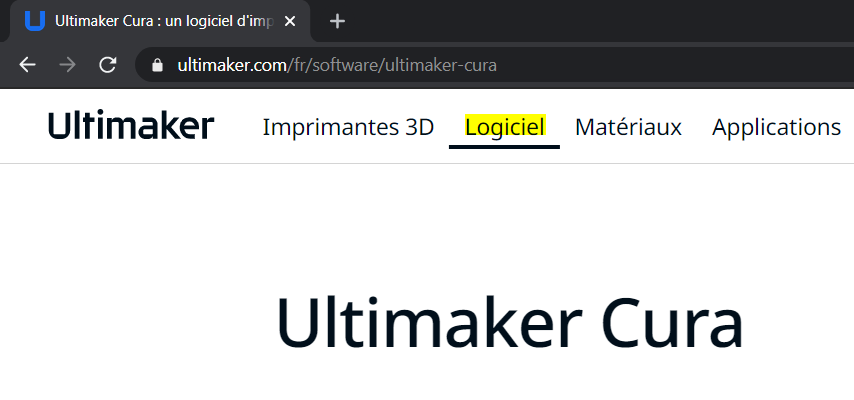
\includegraphics[width=125pt]{Déroulé/Jour_3/TestServo/étape1.PNG}
    \caption{Test servomoteur - \'Etape 1}
    \label{fig:my_label}
\end{figure}

%provisoire
\newpage

\textbullet \, Une fois le servomoteur déposé sur la surface de travail, cliquer sur la petit équerre jusqu'à ce qu'il ait effectué un demi tour sur lui même :
\begin{figure}[!h]
    \centering
    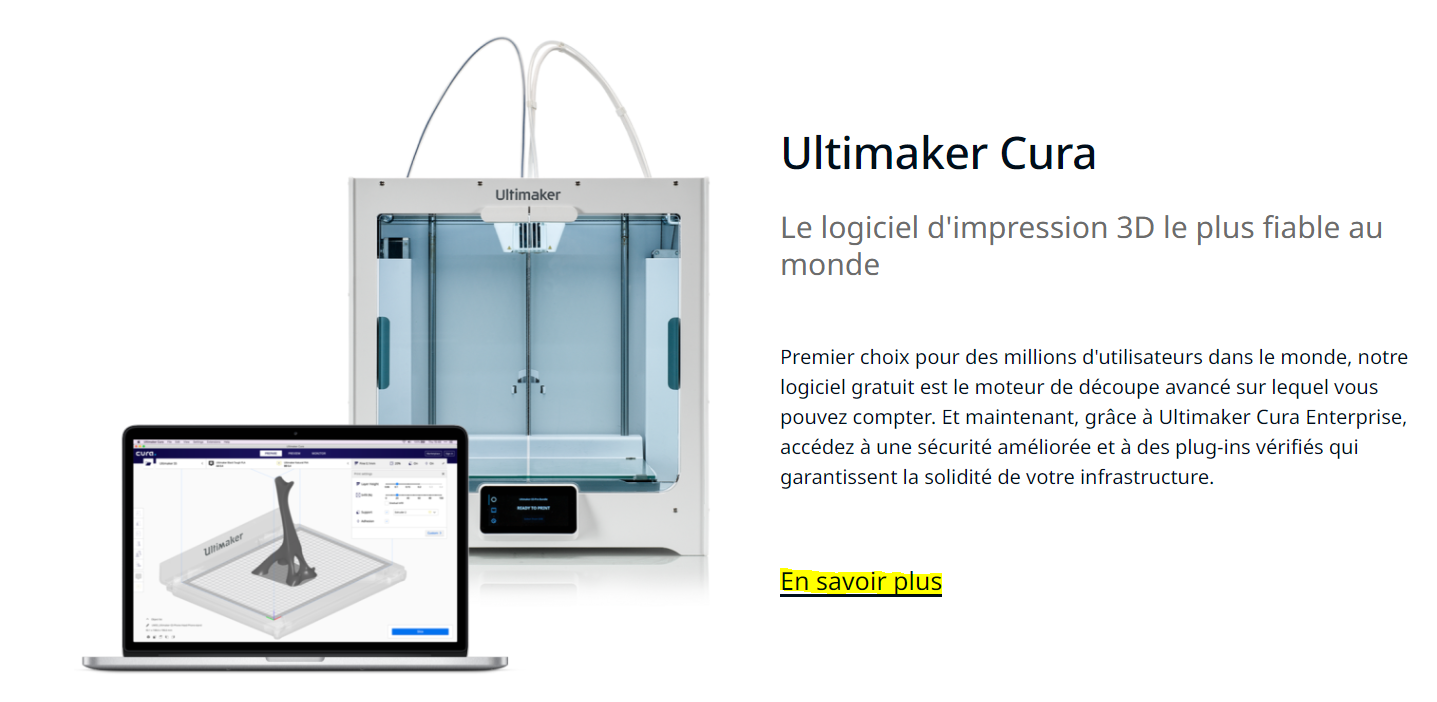
\includegraphics[width=350pt]{Déroulé/Jour_3/TestServo/étape2.PNG}
    \caption[\'Etape 2]{Test servomoteur - \'Etape 2}
    \label{fig:my_label}
\end{figure}

\textbullet \, Ensuite, relier les différents ports du servomoteur comme ci-dessous :
\begin{figure}[!h]
    \centering
    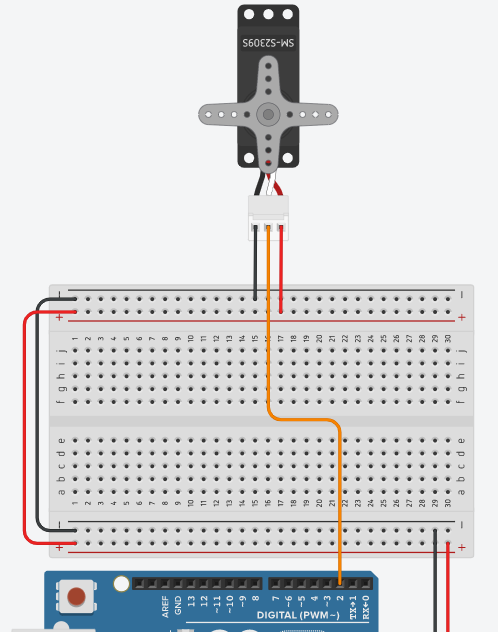
\includegraphics[width=200pt,height=250pt]{Déroulé/Jour_3/TestServo/étape3.PNG}
    \caption[\'Etape 3]{Test servomoteur - \'Etape 3}
    \label{3.18}
\end{figure}

%provisoire
\newpage

\textbullet \, Cliquer sur \textit{Code} :
\begin{figure}[!h]
    \centering
    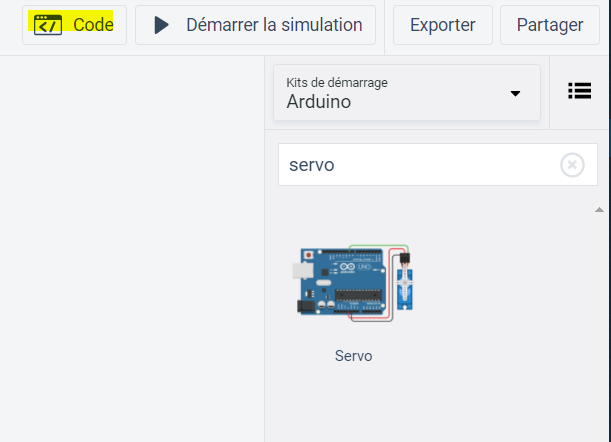
\includegraphics[height=240pt]{Déroulé/Jour_3/TestServo/étape4.PNG}
    \caption[\'Etape 4]{Test servomoteur - \'Etape 4}
    \label{fig:my_label}
\end{figure}

\textbullet \, Aller dans \textit{Blocs + texte}, \textit{Contrôle} cliquer sur \textit{Totaliser..} et déposer le bloc dans l'espace de travail :\\
De nouvelles choses apparaissent sur la portion de l'écran comportant le code
\begin{figure}[!h]
    \centering
    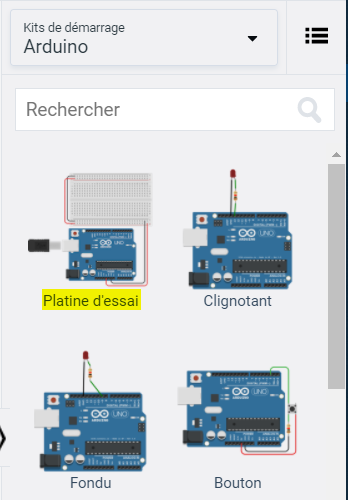
\includegraphics[width=500pt]{Déroulé/Jour_3/TestServo/étape5.PNG}
    \caption[\'Etape 5]{Test servomoteur - \'Etape 5}
    \label{fig:my_label}
\end{figure}

%provisoire
\newpage

\textbullet \, Cliquer sur \textit{i}, \textit{Renommer la variable} et l'appeler \textit{"pos"} :
\begin{figure}[!h]
    \centering
    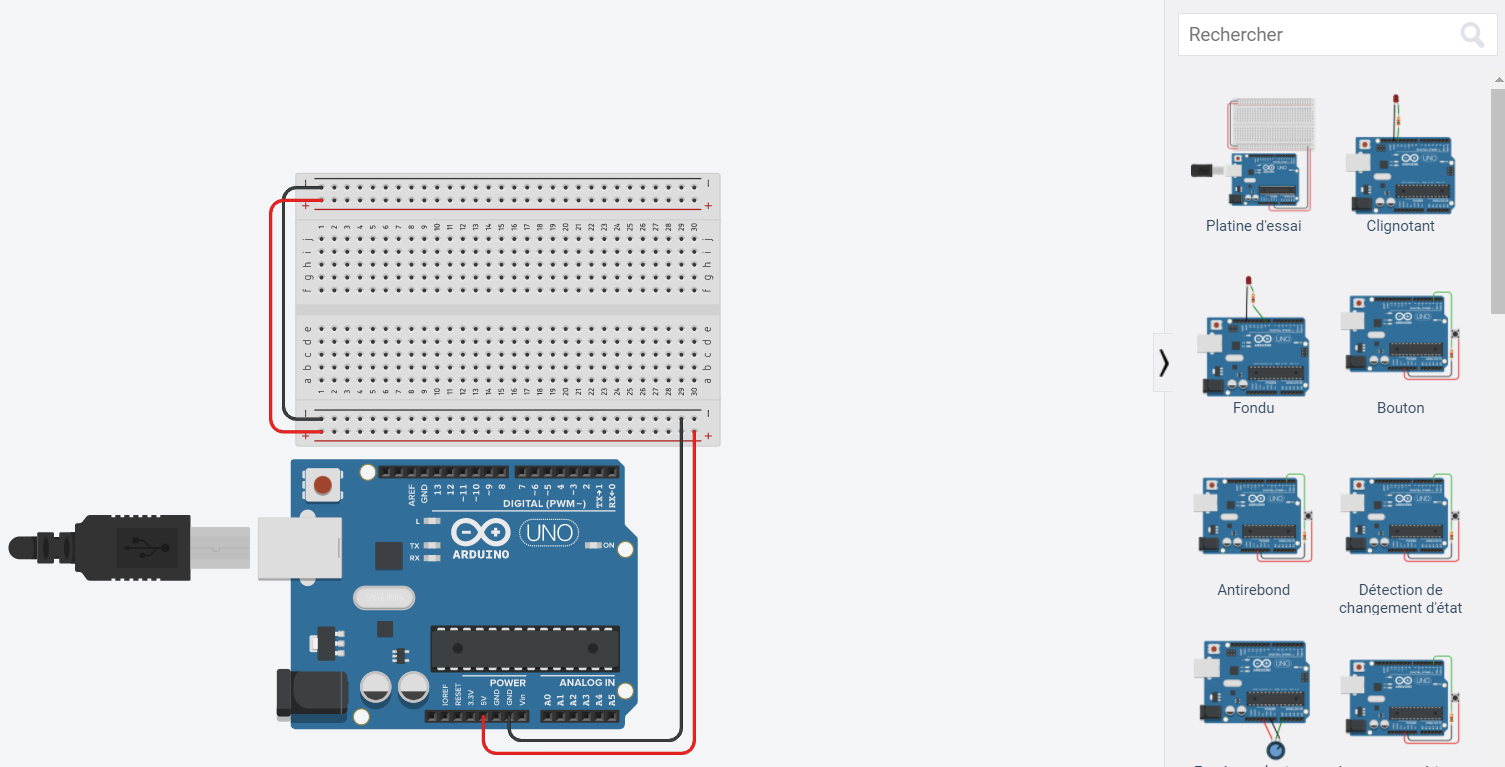
\includegraphics[width=250pt,height=100pt]{Déroulé/Jour_3/TestServo/étape6.PNG}
    \caption[\'Etape 6]{Test servomoteur - \'Etape 6}
    \label{fig:my_label}
\end{figure}

\textbullet \, Retourner dans \textit{Sortie}, cliquer sur \textit{Faire pivoter..} et déposer le bloc dans l'espace de travail :
\begin{figure}[!h]
    \centering
    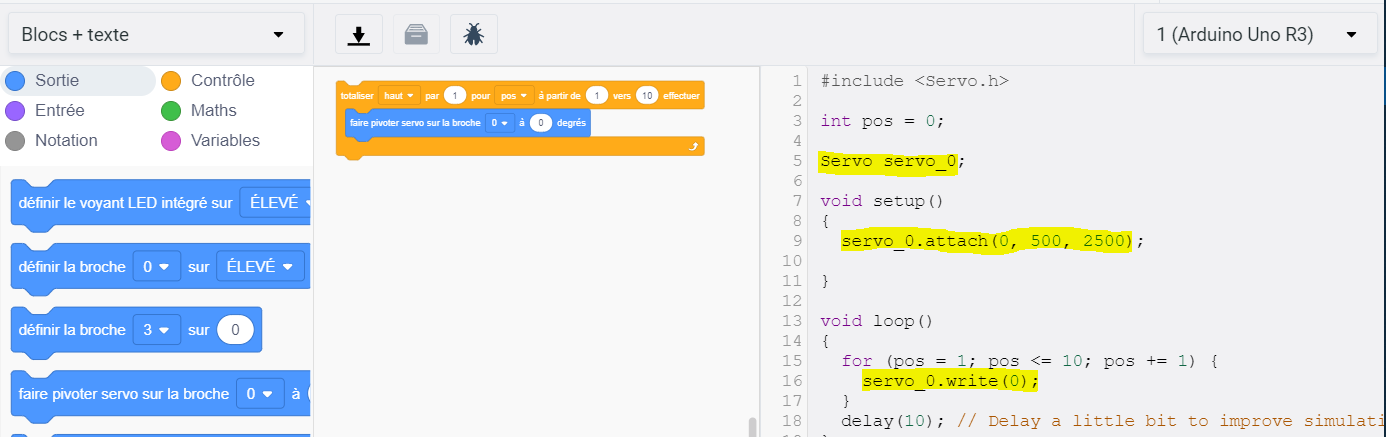
\includegraphics[width=450pt]{Déroulé/Jour_3/TestServo/étape7.PNG}
    \caption[\'Etape 7]{Test servomoteur - \'Etape 7}
    \label{fig:my_label}
\end{figure}

\textbullet \, Retourner dans \textit{Contrôle}, cliquer sur \textit{Patienter} et déposer le bloc dans l'espace de travail :
\begin{figure}[!h]
    \centering
    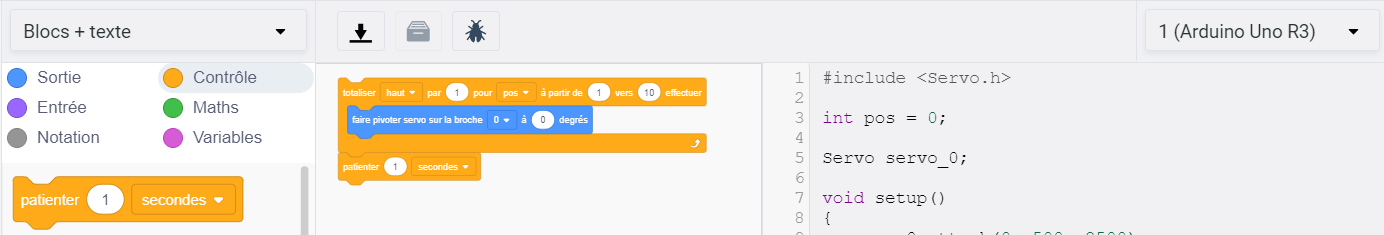
\includegraphics[width=500pt,height=150pt]{Déroulé/Jour_3/TestServo/étape8.PNG}
    \caption[\'Etape 8]{Test servomoteur - \'Etape 8}
    \label{fig:my_label}
\end{figure}

%provisoire
\newpage

\textbullet \, Faire un clic droit sur l'ensemble de blocs, cliquer sur \textit{Dupliquer} et venir positionner le nouveau bloc sous le précédent :
\begin{figure}[!h]
    \centering
    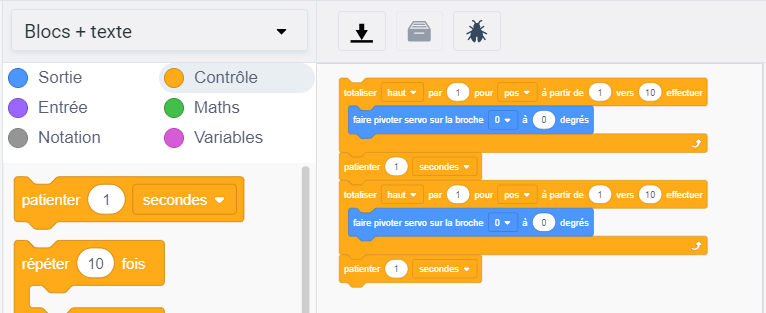
\includegraphics[width=475pt]{Déroulé/Jour_3/TestServo/étape9.PNG}
    \caption[\'Etape 9]{Test servomoteur - \'Etape 9}
    \label{fig:my_label}
\end{figure}

\textbullet \, Modifier les valeurs des blocs comme ci-dessous, voici le code final pour tester le fonctionnement du servomoteur :
\begin{figure}[!h]
    \centering
    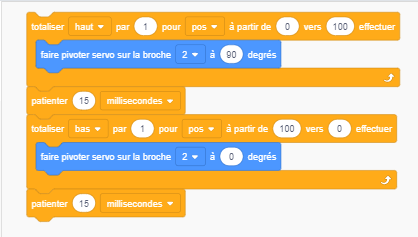
\includegraphics[width=250pt]{Déroulé/Jour_3/TestServo/étape10.PNG}
    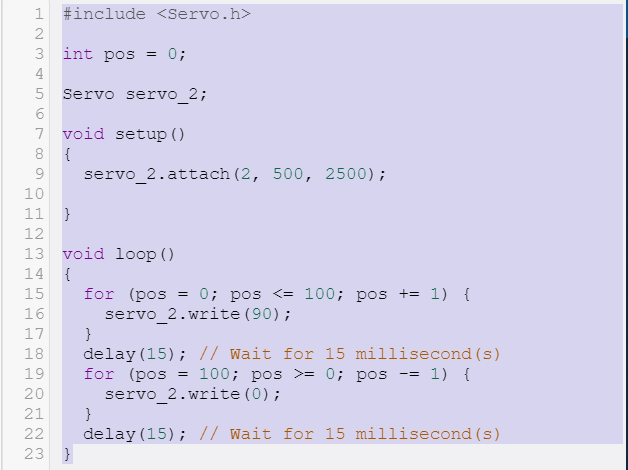
\includegraphics[width=200pt]{Déroulé/Jour_3/TestServo/étape10_1.PNG}
    \caption[\'Etape 10]{Test servomoteur - \'Etape 10}
    \label{fig:my_label}
\end{figure}

%provisoire
\newpage

\textbullet \, Copier/coller votre code dans le logiciel Arduino IDE :\\
Il n'est pas possible de le faire sur Tinkercad lorsque l'on écrit un programme en blocs, il faut donc penser à remplacer les valeurs \textit{0} et \textit{90} par la variable \textit{"pos"}, ainsi qu'enlever la plage de valeur de déplacement du servomoteur qui est optionnelle et ne nous intéresse pas ici.
\begin{figure}[!h]
    \centering
    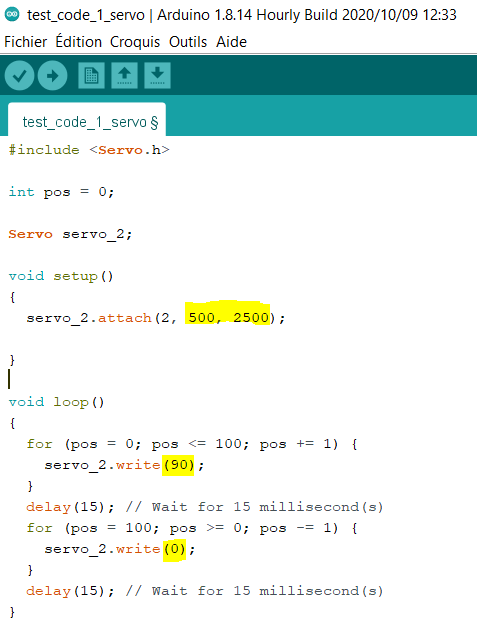
\includegraphics[height=350pt]{Déroulé/Jour_3/TestServo/étape11.PNG}
    \caption[\'Etape 11]{Test servomoteur - \'Etape 11}
    \label{fig:my_label}
\end{figure}

\textbullet \, Effectuer les branchements du servomoteur sur votre carte Arduino (Se référer à la figure \ref{3.18}).\\

%provisoire
\newpage

\textbullet \, Brancher la carte Arduino à l'ordinateur puis cliquer sur \textit{Téléverser} :
\begin{figure}[!h]
    \centering
    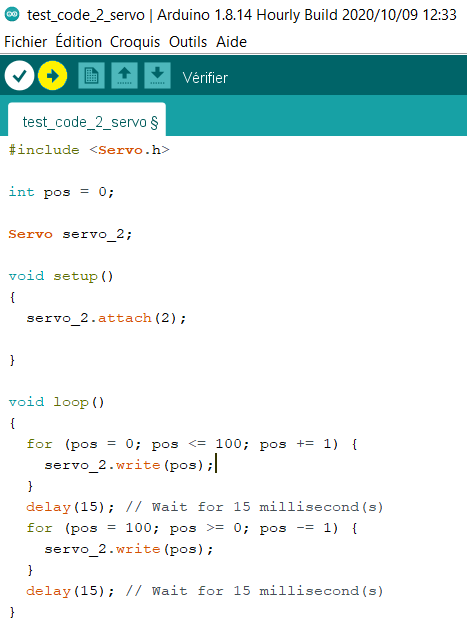
\includegraphics[height=350pt]{Déroulé/Jour_3/TestServo/étape12.PNG}
    \caption[\'Etape 12]{Test servomoteur - \'Etape 12}
    \label{fig:my_label}
\end{figure}

\begin{multicols}{2}
    
\includegraphics[width=80pt,height=80pt]{Déroulé/Jour_1/Manuel d'utilisation/Images/6.jpg}
    
    \columnbreak
    
    \textbf{\large Attention : }\textbf{\textit{Il est possible que vos servomoteurs soient montés à l'envers. Si lorsque vous téléversez le programme sur la carte vous voyez que le servomoteur force, débranchez le, puis inversez le - et le + dans votre programme. Téléversez de nouveau, le servomoteur doit se comporter normalement.}}
\end{multicols}

\end{flushleft}